\documentclass[runningheads]{llncs}
\usepackage[T1]{fontenc}
\usepackage{lmodern}
\usepackage{graphicx}
\usepackage{booktabs}
\usepackage{array}
\newcolumntype{L}[1]{>{\raggedright\arraybackslash}p{#1}}
\usepackage{amsmath}
\usepackage{xurl}
\usepackage{microtype}
\usepackage[hidelinks]{hyperref}
\usepackage{xcolor}
\newcommand{\attack}{ATT\&CK}

\begin{document}

\title{Counting Incidents, Not Reports:\\ Duplicate-Coverage Bias in {ATT\&CK} Technique Statistics}
\titlerunning{Counting Incidents, Not Reports}
\author{Anonymous Author(s)}
\authorrunning{Anonymous}
\institute{Withheld for review}

\maketitle

\begin{abstract}
Rankings of the most common \attack{} techniques are built by counting threat reports. When a high-profile intrusion is written up by many vendors, it is counted many times. We measure this duplicate-coverage bias by counting each incident once instead of each report, on three corpora: 1,936 reports cited by MITRE \attack{} v20.1, 6,025 TIE/OpenCTI report entries, and 3,775 public report texts (532 with explicit technique IDs). Incidents are formed by a constrained clustering rule: a shared subject actor or malware within 60 days, or three shared rare indicators, with commodity tools excluded and a 60-day span cap. On \attack{}'s own campaign assignments the rule makes no false merges and recovers 39\% of same-campaign pairs. The two-month rule used in prior work does as well on curated \attack{} metadata but collapses on full report texts, where one cluster absorbs 1,375 reports. The top of the ranking is stable (Kendall $\tau_b$ 0.97--0.99; the top-20 changes by at most one technique), but the middle is not. In \attack{}, per-report counting overstates the share of Data Encrypted for Impact by 22\% (95\% CI 12--35\%), of Data Destruction by 36\%, and of supply-chain and token-theft techniques by about 86\%, worth up to 74 rank places. In 2026, four of the ten most cited techniques are artefacts of a single supply-chain campaign. A second correction that weights every vendor equally moves a different set of techniques (rank correlation with the duplicate effect $\approx 0$), so producer volume and duplicate coverage are separate biases. A permutation null confirms that the over-counting comes from repeated coverage, not from incident size alone. We release code and per-technique results.

\keywords{Cyber threat intelligence \and MITRE ATT\&CK \and Measurement \and Reporting bias \and Deduplication}
\end{abstract}

\section{Introduction}

Defenders use technique frequency to decide what to detect first. Vendor ``top techniques'' lists, \attack{}-based prioritisation calculators~\cite{ctid2022top} and academic studies~\cite{rahman2024arsenal} count how often each technique appears across threat intelligence reports. The unit of counting is the report. Reports are not independent observations of attacker behaviour, however. The SolarWinds compromise, the Ryuk/TrickBot wave of 2020, Black Basta and the 2026 TeamPCP supply-chain campaign were each described by 9 to 12 separate reports cited by \attack{}, while most intrusions are described once or never. Per-report counting therefore weights a technique by how newsworthy the incidents that used it were, not by how often attackers used it.

This bias is widely acknowledged. The \attack{} team, the CTID Sightings report and CISA's mapping guide name availability, novelty and producer bias~\cite{strom2020attack,ctid2021sightings,cisa2023mapping}, and political-science work shows that commercial reporting over-represents high-profile actors~\cite{maschmeyer2021tale}. It has not been measured for technique statistics. The closest work deduplicates \attack{} citations with a rule (same group or malware within two months) but neither validates the rule nor reports how much it changes the result~\cite{rahman2024arsenal}. We ask:

\begin{itemize}
\item[\textbf{RQ1}] How much does counting incidents instead of reports change technique rankings and shares?
\item[\textbf{RQ2}] Which techniques are over-counted, and why?
\item[\textbf{RQ3}] Is the duplicate-coverage effect distinct from producer bias, that is, from some vendors simply publishing more?
\end{itemize}

\noindent Our contributions are:
\begin{itemize}
\item a constrained incident-clustering rule for threat reports, validated only against independent ground truth (\attack{} campaign assignments and the dated campaign folders of a public report collection), and evidence that the rule used in prior work, while adequate on curated citation metadata, chains unrelated reports on full texts;
\item the first measurement of duplicate-coverage bias in technique statistics, on three corpora, with a cluster bootstrap that identifies significantly over-counted techniques;
\item a decomposition showing that duplicate coverage and producer volume shift different techniques;
\item a worked example on yearly top-10 lists, and released code and per-technique results.
\end{itemize}

The approach needs no labelling, no language model and no GPU, so it can be rerun on every new \attack{} release.

\section{Related Work}

\paragraph{Technique frequency.} Rahman et al.~\cite{rahman2024arsenal} mine \attack{} v12 citations for the most common techniques and technique sequences. They treat two citations as one incident if they share a group or malware and were published within two months, reducing 920 citations to 667; the rule is assumed rather than validated, and results without it are not reported. We find that it works on \attack{}'s curated metadata but not on full texts (Sect.~\ref{sec:val}). Cyentia and Tidal Cyber~\cite{cyentia2023multisource} compare 22 public top-technique lists and find wide disagreement: about a third of techniques are never mentioned. The CTID Sightings project~\cite{ctid2021sightings} counts technique detections contributed by security vendors rather than reports, and its Top \attack{} Techniques calculator weights prevalence from those sightings~\cite{ctid2022top}. Detection-based reports face their own unit-of-counting choice: Red Canary counts each detection towards technique prevalence but counts threats by affected environments~\cite{redcanary2026tdr}. Our work makes the same choice explicit for report-based statistics and measures its effect.

\paragraph{Bias in threat reporting.} Maschmeyer et al.~\cite{maschmeyer2021tale} show that commercial reports focus on high-end threats to well-resourced targets and under-represent threats to civil society. Furumoto et al.~\cite{furumoto2025survey} survey 200+ CTI studies and warn that datasets built from major vendors' reports inherit source and regional biases. Suarez-Roman et al.~\cite{suarezroman2026echo} structure 13,308 reports with a language model and measure vendor overlap and specificity; they remove identical documents but do not cluster incidents or test the effect on technique statistics. For indicator feeds, Li et al.~\cite{li2019tealeaves} and Bouwman et al.~\cite{bouwman2020cup} find little overlap between feeds and question their coverage. These works characterise who reports what; none quantifies how repeated coverage of the same incident distorts aggregate technique statistics, or separates it from producer volume.

\paragraph{Linking reports.} Knowledge-graph and deduplication pipelines link reports through shared indicators or entities. We use the same signals, but show that without guards against transitive chaining, entity-based linking merges unrelated reports, which is the main failure mode for counting.

\section{Data}

We use three corpora that differ in who chose the reports and how techniques were assigned (Table~\ref{tab:data}). No labelling, language model or GPU is used.

\begin{table}[t]
\caption{Corpora. ``Units'' are the per-report counting units.}\label{tab:data}
\centering\footnotesize
\setlength\tabcolsep{4pt}
\begin{tabular}{@{}L{2.1cm}L{1.6cm}L{3.2cm}L{4.4cm}@{}}
\toprule
Corpus & Units & Technique labels & Dates and entities \\
\midrule
\attack{} v20.1 citations & 1,936 & techniques the report is cited for in \emph{uses} relations & date in the citation (1,839 dated); groups, software and campaigns the citation supports \\
TIE / OpenCTI~\cite{turner2025tie} & 6,025 & TIE technique sets & OTX pulse metadata (305 entries) or vendor URL; 1,564 dated \\
Report texts & 3,775; 532 with $\geq$3 IDs & explicit technique IDs in the text & page date, folder date or advisory number; \attack{} alias matches; indicators \\
\bottomrule
\end{tabular}
\end{table}

The text corpus combines vendor blog posts, the public APT \& CyberCriminal Campaign Collections~\cite{cybermonitor2024apt} (reports filed in dated campaign folders, 2006--2024), and 314 CISA AA/AR advisories from 2018 to 2026, of which 186 were not already present. Pages on attack.mitre.org are excluded because they summarise many reports. Indicators are file hashes, public IP addresses and defanged domains. \attack{} is the most curated corpus and the most relevant to practice, since prioritisation tools count its citations. TIE is the largest, but only 26\% of its entries could be dated, so its results are a lower bound on the effect.

\section{Method}

\subsection{Incident clustering}

Two reports are linked when (a) they share a subject actor, campaign or malware and were published at most $\tau = 60$ days apart, or (b) they share at least three rare indicators, each seen in 2 to 20 reports. Incidents are groups of linked reports. Three guards prevent the chaining that defeats naive linking:

\begin{enumerate}
\item \textbf{Commodity tools never link.} Software that \attack{} lists for four or more groups (51 items, such as Cobalt Strike, Mimikatz and PsExec) is ignored.
\item \textbf{Only the subject counts.} In a text, an entity is a subject if it is named at least three times and at least half as often as the most-named entity (at most two per report). Overview reports with more than eight such entities get no entity links. Reports dated only to a year link only through indicators.
\item \textbf{Constrained single linkage.} Links are merged in order of strength (indicator links first, then shortest time gap). A merge is refused if the resulting incident would span more than $S = 60$ days.
\end{enumerate}

In \attack{}, entities are the objects a citation supports; in TIE, they come from OTX pulse fields and the vendor URL.

\subsection{Counting and comparison}

Per-report counting adds one for each report that mentions a technique; per-incident counting adds one for each incident in which any report mentions it. We compare rankings with Kendall's $\tau_b$ on technique shares and with top-$k$ overlap. For technique $t$ with per-report count $R(t)$ and per-incident count $I(t)$, the share ratio is
\begin{equation}
\rho(t) = \frac{R(t) / \sum_u R(u)}{I(t) / \sum_u I(u)} .
\end{equation}
$\rho(t) > 1$ means that per-report counting overstates $t$'s share. A 95\% interval comes from a cluster bootstrap that resamples incidents (1,000 replicates); $t$ is over-counted when the whole interval lies above 1. Techniques with fewer than 20 report mentions (15 in the text corpus) are not tested. Because frequent techniques recur in any large incident, we also compare $\rho$ with a permutation null: 200 random incident assignments that keep the incident-size distribution and shuffle reports only within their publication year. A technique that appears only in single-report incidents has $\rho = \sum I / \sum R$ (0.90 in \attack{}), the baseline against which over-counting is measured.

\subsection{Producer correction}

To separate duplicate coverage from producer volume, we also weight each report by $1/n(v)$, where $n(v)$ is the number of reports from its vendor $v$, so that every vendor counts once. The producer ratio is the per-report share over this vendor-balanced share, with a bootstrap over vendors. Vendors are taken from the report URL's domain (archived copies are mapped to the original site); texts without a URL count as their own vendor.

\section{Validation on Independent Ground Truth}\label{sec:val}

We validate only against groupings made by others, independently of this study:

\begin{itemize}
\item \textbf{\attack{} campaigns.} 59 cited reports that support exactly one \attack{} campaign and also name a group or malware, in 33 campaigns (69 same-campaign pairs). Campaign links are removed before clustering, so the rule cannot use the answer.
\item \textbf{Campaign folders.} The report collection~\cite{cybermonitor2024apt} files reports in dated folders, one per campaign or publication event. 97 folders hold two or more texts (212 same-folder pairs). Separate folders sometimes hold the same campaign, so precision here is a lower bound.
\end{itemize}

\begin{table}[t]
\caption{Pairwise precision (P) and recall (R) against independent ground truth. $\tau$: maximum gap between linked reports; $S$: maximum incident span. Folder precision is a lower bound.}\label{tab:val}
\centering\footnotesize
\begin{tabular}{@{}lcccc@{}}
\toprule
 & \multicolumn{2}{c}{\attack{} campaigns} & \multicolumn{2}{c}{Campaign folders} \\
Setting & P & R & P (lower bound) & R \\
\midrule
$\tau = 60$, $S = 60$ (main) & 1.00 & 0.39 & 0.25 & 0.59 \\
$\tau = 60$, $S = 45$ & 1.00 & 0.32 & 0.29 & 0.59 \\
$\tau = 60$, $S = 180$ & 1.00 & 0.41 & 0.18 & 0.59 \\
$\tau = 0$ (same day) & 1.00 & 0.09 & -- & -- \\
$\tau = 60$, no span cap & 1.00 & 0.41 & 0.01 & 0.59 \\
Prior rule~\cite{rahman2024arsenal}: $\tau = 60$, no guards & 1.00 & 0.41 & 0.001 & 0.73 \\
No time limit & 0.45 & 0.48 & -- & -- \\
\bottomrule
\end{tabular}
\end{table}

Table~\ref{tab:val} shows that on \attack{}'s curated metadata, where each citation is linked only to the groups and software it supports, any rule with a time window works: the prior rule and ours both make no false merges. Without a time window, single linkage chains reports through shared actors over years and the largest \attack{} cluster grows from 12 to 477 reports. Full texts are different, because they mention many actors and tools in passing. There the prior rule merges 1,375 of 3,775 texts into one cluster (folder precision 0.001), and even with our subject and commodity-tool guards, removing the span cap grows the largest cluster from 12 to 275. We fix $S = 60$: it keeps \attack{} recall at 0.39 while raising folder precision from 0.18 ($S = 180$) to 0.25; $S = 45$ gains a little precision at a larger loss of recall. $S \in \{45, 90, 180, 365\}$ are reported as sensitivity checks.

Recall of 0.39 means that many same-campaign reports stay separate, mostly follow-up analyses published months after the first wave. Under-merging pulls per-incident counts towards per-report counts, so the over-counting we report is conservative.

\section{Results}

\subsection{RQ1: The top is stable, the middle is not}

Counting incidents leaves the top of every ranking almost unchanged (Table~\ref{tab:rq1}). In \attack{}, 810 of 1,936 cited reports (42\%) fall into 302 multi-report incidents, yet $\tau_b$ is 0.97 and the top-20 is identical. Across all settings of Table~\ref{tab:val} except the unconstrained rule, \attack{} $\tau_b$ stays between 0.96 and 0.997 and top-20 overlap at 19 or 20; linking on shared actors with no time window gives $\tau_b = 0.905$ and overlap 17, and the prior rule applied to full texts gives $\tau_b = 0.853$ and overlap 14. The choice of clustering rule therefore changes the answer more than the decision to deduplicate.

\begin{table}[t]
\caption{Per-report vs.\ per-incident rankings (technique level, $\tau = S = 60$).}\label{tab:rq1}
\centering\footnotesize\setlength\tabcolsep{6pt}
\begin{tabular}{@{}lrrcccc@{}}
\toprule
Corpus & Reports & Incidents & $\tau_b$ & Top-10 & Top-20 & Top-50 \\
\midrule
\attack{} citations & 1,936 & 1,428 & 0.970 & 9 & 20 & 49 \\
Report texts with T-IDs & 532 & 470 & 0.990 & 10 & 19 & 49 \\
TIE / OpenCTI$^{a}$ & 6,025 & 5,442 & 0.992 & 10 & 19 & 50 \\
\bottomrule
\multicolumn{7}{@{}l}{\scriptsize $^{a}$ 5,596 distinct reports after merging entries that point to the same vendor URL.}
\end{tabular}
\end{table}

\subsection{RQ2: What is over-counted}

\begin{figure}[t]
\centering
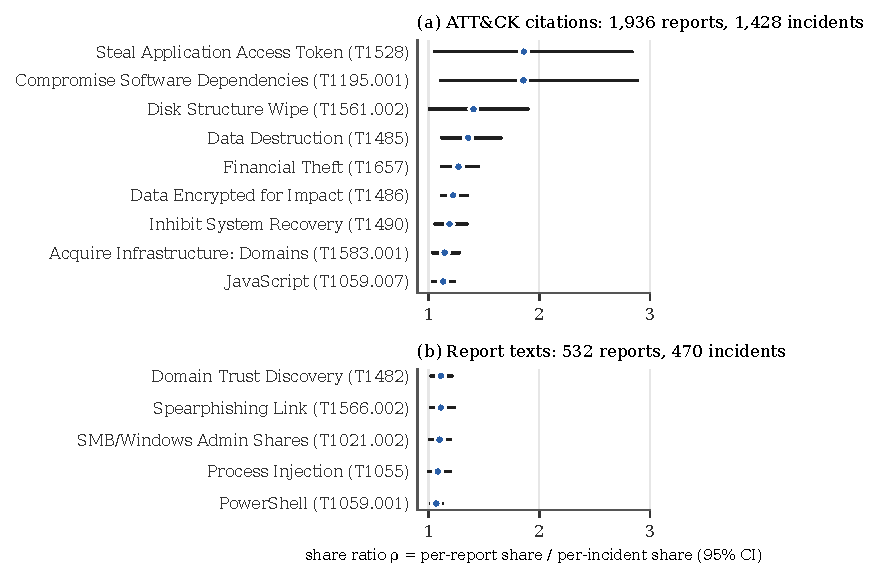
\includegraphics[width=0.95\textwidth]{fig_share_ratio.pdf}
\caption{Techniques whose share is significantly overstated by per-report counting (95\% cluster-bootstrap interval above 1). (a) \attack{}: the nine that also exceed a permutation null (six generic techniques with $\rho$ 1.04--1.07 do not and are omitted). (b) All five in the report texts.}\label{fig:rho}
\end{figure}

In \attack{} the significantly over-counted techniques are destructive and supply-chain techniques (Fig.~\ref{fig:rho}a). Steal Application Access Token and Compromise Software Dependencies have $\rho \approx 1.86$ and fall from rank 166 to 240 and 160 to 228; Disk Structure Wipe ($\rho = 1.41$), Data Destruction (1.36, rank 88 to 114), Financial Theft (1.27, 78 to 101), Data Encrypted for Impact (1.22, 30 to 37) and Inhibit System Recovery (1.19, 59 to 70) follow. They come from a few heavily covered events: SolarWinds (12 reports in one incident), the Ryuk/TrickBot wave of autumn 2020 (9), two TeamPCP waves in 2026 (9 and 7), Black Basta (9), VOID MANTICORE (8) and WhisperGate (6). Six frequent generic techniques, such as Ingress Tool Transfer and Web Protocols, also have intervals just above 1 ($\rho$ 1.04--1.07). The permutation null explains them: shuffling reports into incidents of the same sizes gives the same ratios ($p \geq 0.07$), because a frequent technique is likely to repeat inside any large incident. The nine techniques of Fig.~\ref{fig:rho}a exceed the null in all 200 permutations, so their excess comes from which incidents were covered repeatedly. Eight of the nine stay significant at every span cap from 45 days to no cap.

In the report texts the over-counted techniques are hands-on-keyboard intrusion steps (Fig.~\ref{fig:rho}b): Domain Trust Discovery, Spearphishing Link, SMB/Windows Admin Shares, Process Injection and PowerShell ($\rho$ 1.07--1.11; PowerShell drops from rank 2 to 4). They come from CISA and The DFIR Report publishing several reports on the same ransomware crews within weeks. In TIE the shifts are small ($\rho \leq 1.05$) because few entries could be linked.

\subsection{Effect on a published-style statistic}

We rebuild a yearly top-10 from \attack{} citations for every year with at least 60 cited reports (2015--2026). Per-incident counting changes the top-10 in 8 of 12 years, 13 entries in total. The clearest case is 2026 (Fig.~\ref{fig:2026}): 67 cited reports form 26 incidents, and four of the per-report top-10 drop to ranks 34 to 64. All four come from the TeamPCP campaign. A 2026 top-techniques list built from citations would describe one campaign, not the year.

\begin{figure}[t]
\centering
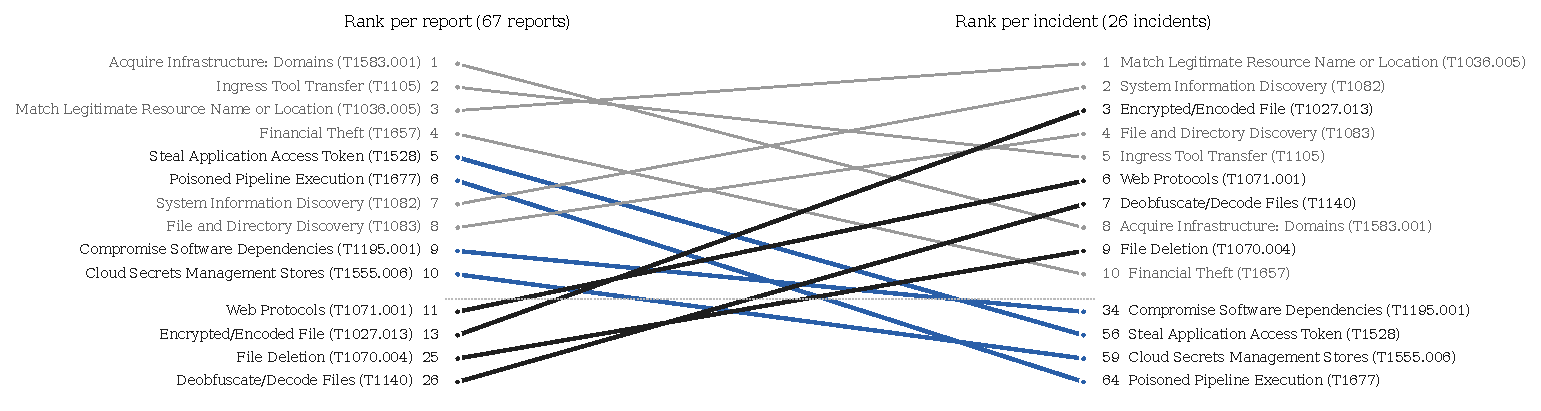
\includegraphics[width=\textwidth]{fig_2026_top10.pdf}
\caption{\attack{} techniques cited in 2026, ranked per report (left) and per incident (right). Blue: techniques that leave the top-10, all from the TeamPCP supply-chain campaign. Black: techniques that enter it. Grey: techniques in both top-10s.}\label{fig:2026}
\end{figure}

\subsection{RQ3: Duplicate coverage is not producer bias}

The vendor-balanced correction moves a different set of techniques. Across the 215 tested \attack{} techniques, the Spearman correlation between the share ratio and the producer ratio is $-0.03$ (0.005 across 196 techniques in the texts). The two corrections can even point in opposite directions. Financial Theft and Steal Application Access Token are over-counted per report ($\rho$ 1.27 and 1.86) but under-represented relative to an equal-vendor view (producer ratio 0.68 and 0.53, intervals below 1), because many small vendors each wrote about them once. Disk Structure Wipe is inflated by both: a few vendors wrote much of the wiper coverage (producer ratio 3.15), and the same wiper events were covered repeatedly. In the texts, the producer effect dominates for ransomware: Financial Theft, Inhibit System Recovery and Data Encrypted for Impact have producer ratios of 3 to 19, because CISA and The DFIR Report contribute most of their mentions. Deduplicating incidents and balancing vendors are therefore both needed, and neither substitutes for the other.

\section{Discussion and Threats to Validity}

\paragraph{Implications.} Top-10 lists built from citations are safe to use as they are. Mid-ranked techniques, the ones that decide what to detect after the obvious, are not: ransomware impact, wiper and supply-chain techniques look more common per report than per incident. Tools that rank techniques by citation count should count incidents and show both views, and a list for a single year or any short window should be checked for single-campaign artefacts.

\paragraph{Incident or episode.} The rule joins reports on the same actor and malware within 60 days. For incident-response blogs this can join separate intrusions by the same crew, so our incidents are closest to campaign waves.

\paragraph{Validation.} Both independent sets are small (69 and 212 positive pairs), recall on \attack{} campaigns is 0.39, and folder precision is only a lower bound. Under-merging makes the estimates conservative. A larger independent gold set, such as vendor campaign identifiers, would tighten them.

\paragraph{Labels and entities.} \attack{} cites a report only for some behaviours, so per-report technique sets are partial; this affects absolute shares more than the comparison. Report texts contribute only explicit technique IDs, which favours recent CISA, DFIR and vendor reports. Actor and malware names are matched to \attack{} aliases; short aliases that are common words caused false matches (``Page'' for Elise, ``Play'' for Playcrypt) and are stop-listed, but some noise remains.

\paragraph{Coverage and vendors.} Only 26\% of TIE entries are dated, so most cannot be linked and TIE results are a lower bound. Vendor identity comes from URL domains; texts without a URL are left unweighted rather than down-weighted.

\section{Conclusion}

Counting each incident once instead of each report leaves the most common \attack{} techniques in place, but shows that per-report counting overstates the share of destructive and supply-chain techniques by 19 to 86\%, worth up to 74 rank places. A validated, constrained clustering rule is essential: on full texts, the rule used before chains unrelated reports and changes rankings more than deduplication itself. Duplicate coverage and producer volume are separate biases that move different techniques, so technique statistics should correct for both.

\paragraph{Artefacts.} Code, per-technique results and cluster assignments: \url{https://anonymous.4open.science/r/counting-incidents-898F/}. Report texts are not redistributed; scripts rebuild the features from the public sources.

\bibliographystyle{splncs04}
\bibliography{refs}

\end{document}
